In this chapter we will go into the structural nature and coming-together of this thesis project. The thesis follows an approach to research practise called Research through Design (RtD). Starting with a listing and outline of all activities that have been done, followed by documentation of the design moves and rationale for these moves throughout the project.


\section{Joint forces with two research buddies}
This thesis is based on quite extensive amounts of fieldwork and design activities that has been made possible because of a joint effort with two other master-students; Janni Rasmussen and Anh Thy Sandra Nguyen. In this thesis they are referred to as my research buddies. We all chose the same thesis outline, but writes separately and have developed our own research agendas. In the early stages we worked together in terms of getting to know the domain and context, for the most part discussing and sharing literature insights. Already during the spring 2021 we started to single out different areas of interests. Regardless of that we have conducted almost all fieldwork together, yet with separate datagathering guides.

\begin{figure}[H]
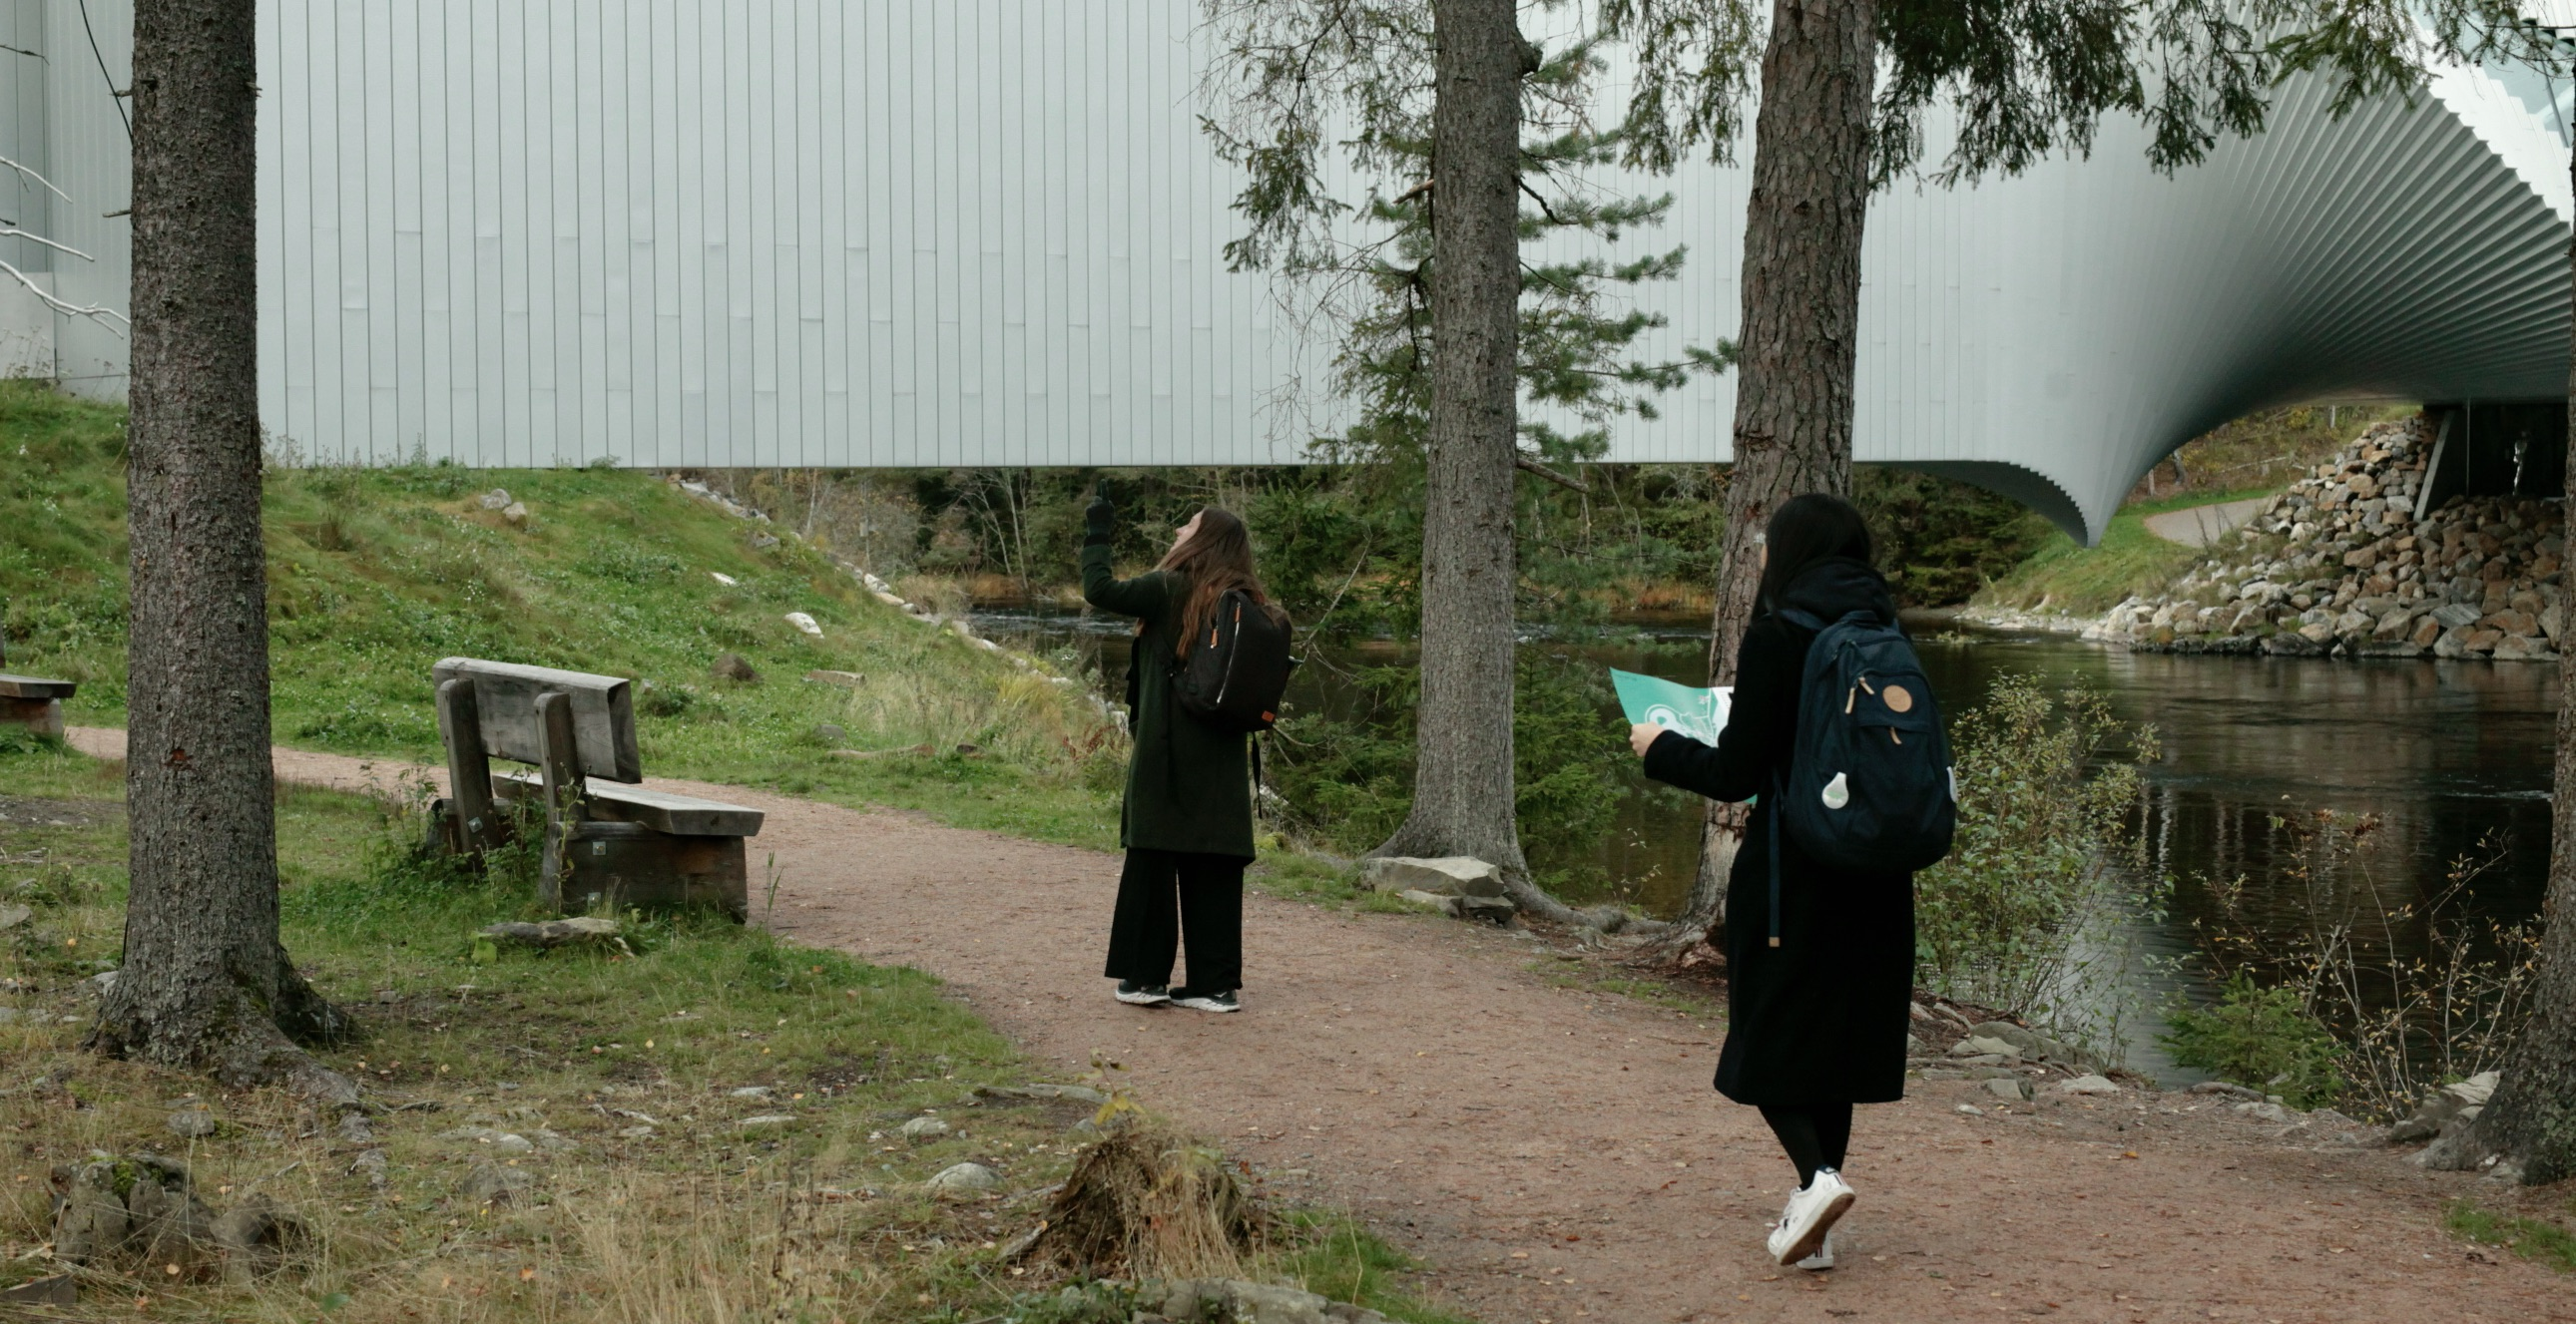
\includegraphics[width=12.3cm]{pictures/methodology/buddies.JPG}
\caption{The research buddies}
\centering 
\end{figure}

Janni is writing about engaging experiences with interactive installations in museums and exhibit spaces, and how engagement can be facilitated with Tangible Interaction. In Sandra's study, she looks into how visitor engagement can be increased through narrative exhibitions, and proposes principles for creating engaging interactive installations in exhibition spaces.


\section{Collaborating with Klimahuset}
The original thesis outline; \emph{interactive and visual installations addressing sustainability}, mentioned Klimahuset as a potential collaboration partner. Klimahuset is a part of University of Oslo: the Natural History Museum. The museum is located in the Botanical Garden at Tøyen, Oslo. Klimahuset represents the type of space where discourses on sustainability matters can take place, available to citizens as a museum. It is newly opened, particularly aimed at young adults aged 14-16. It will be the main space where me and my research buddies will conduct research activities and investigate sustainability issues such as Earth’s climate systems, consequences of global warming, solutions, and what actions individuals can do to contribute to a sustainable transition and future. An important note to the collaboration is that even though some research activities is conducted at Klimahuset, and the end-exhibition will take place there, the end-installation is not supposed to be an artefact designed for Klimahuset. Klimahuset simply provides the contextual space for learning and discussing sustainability-related topics.

\begin{figure}[H]
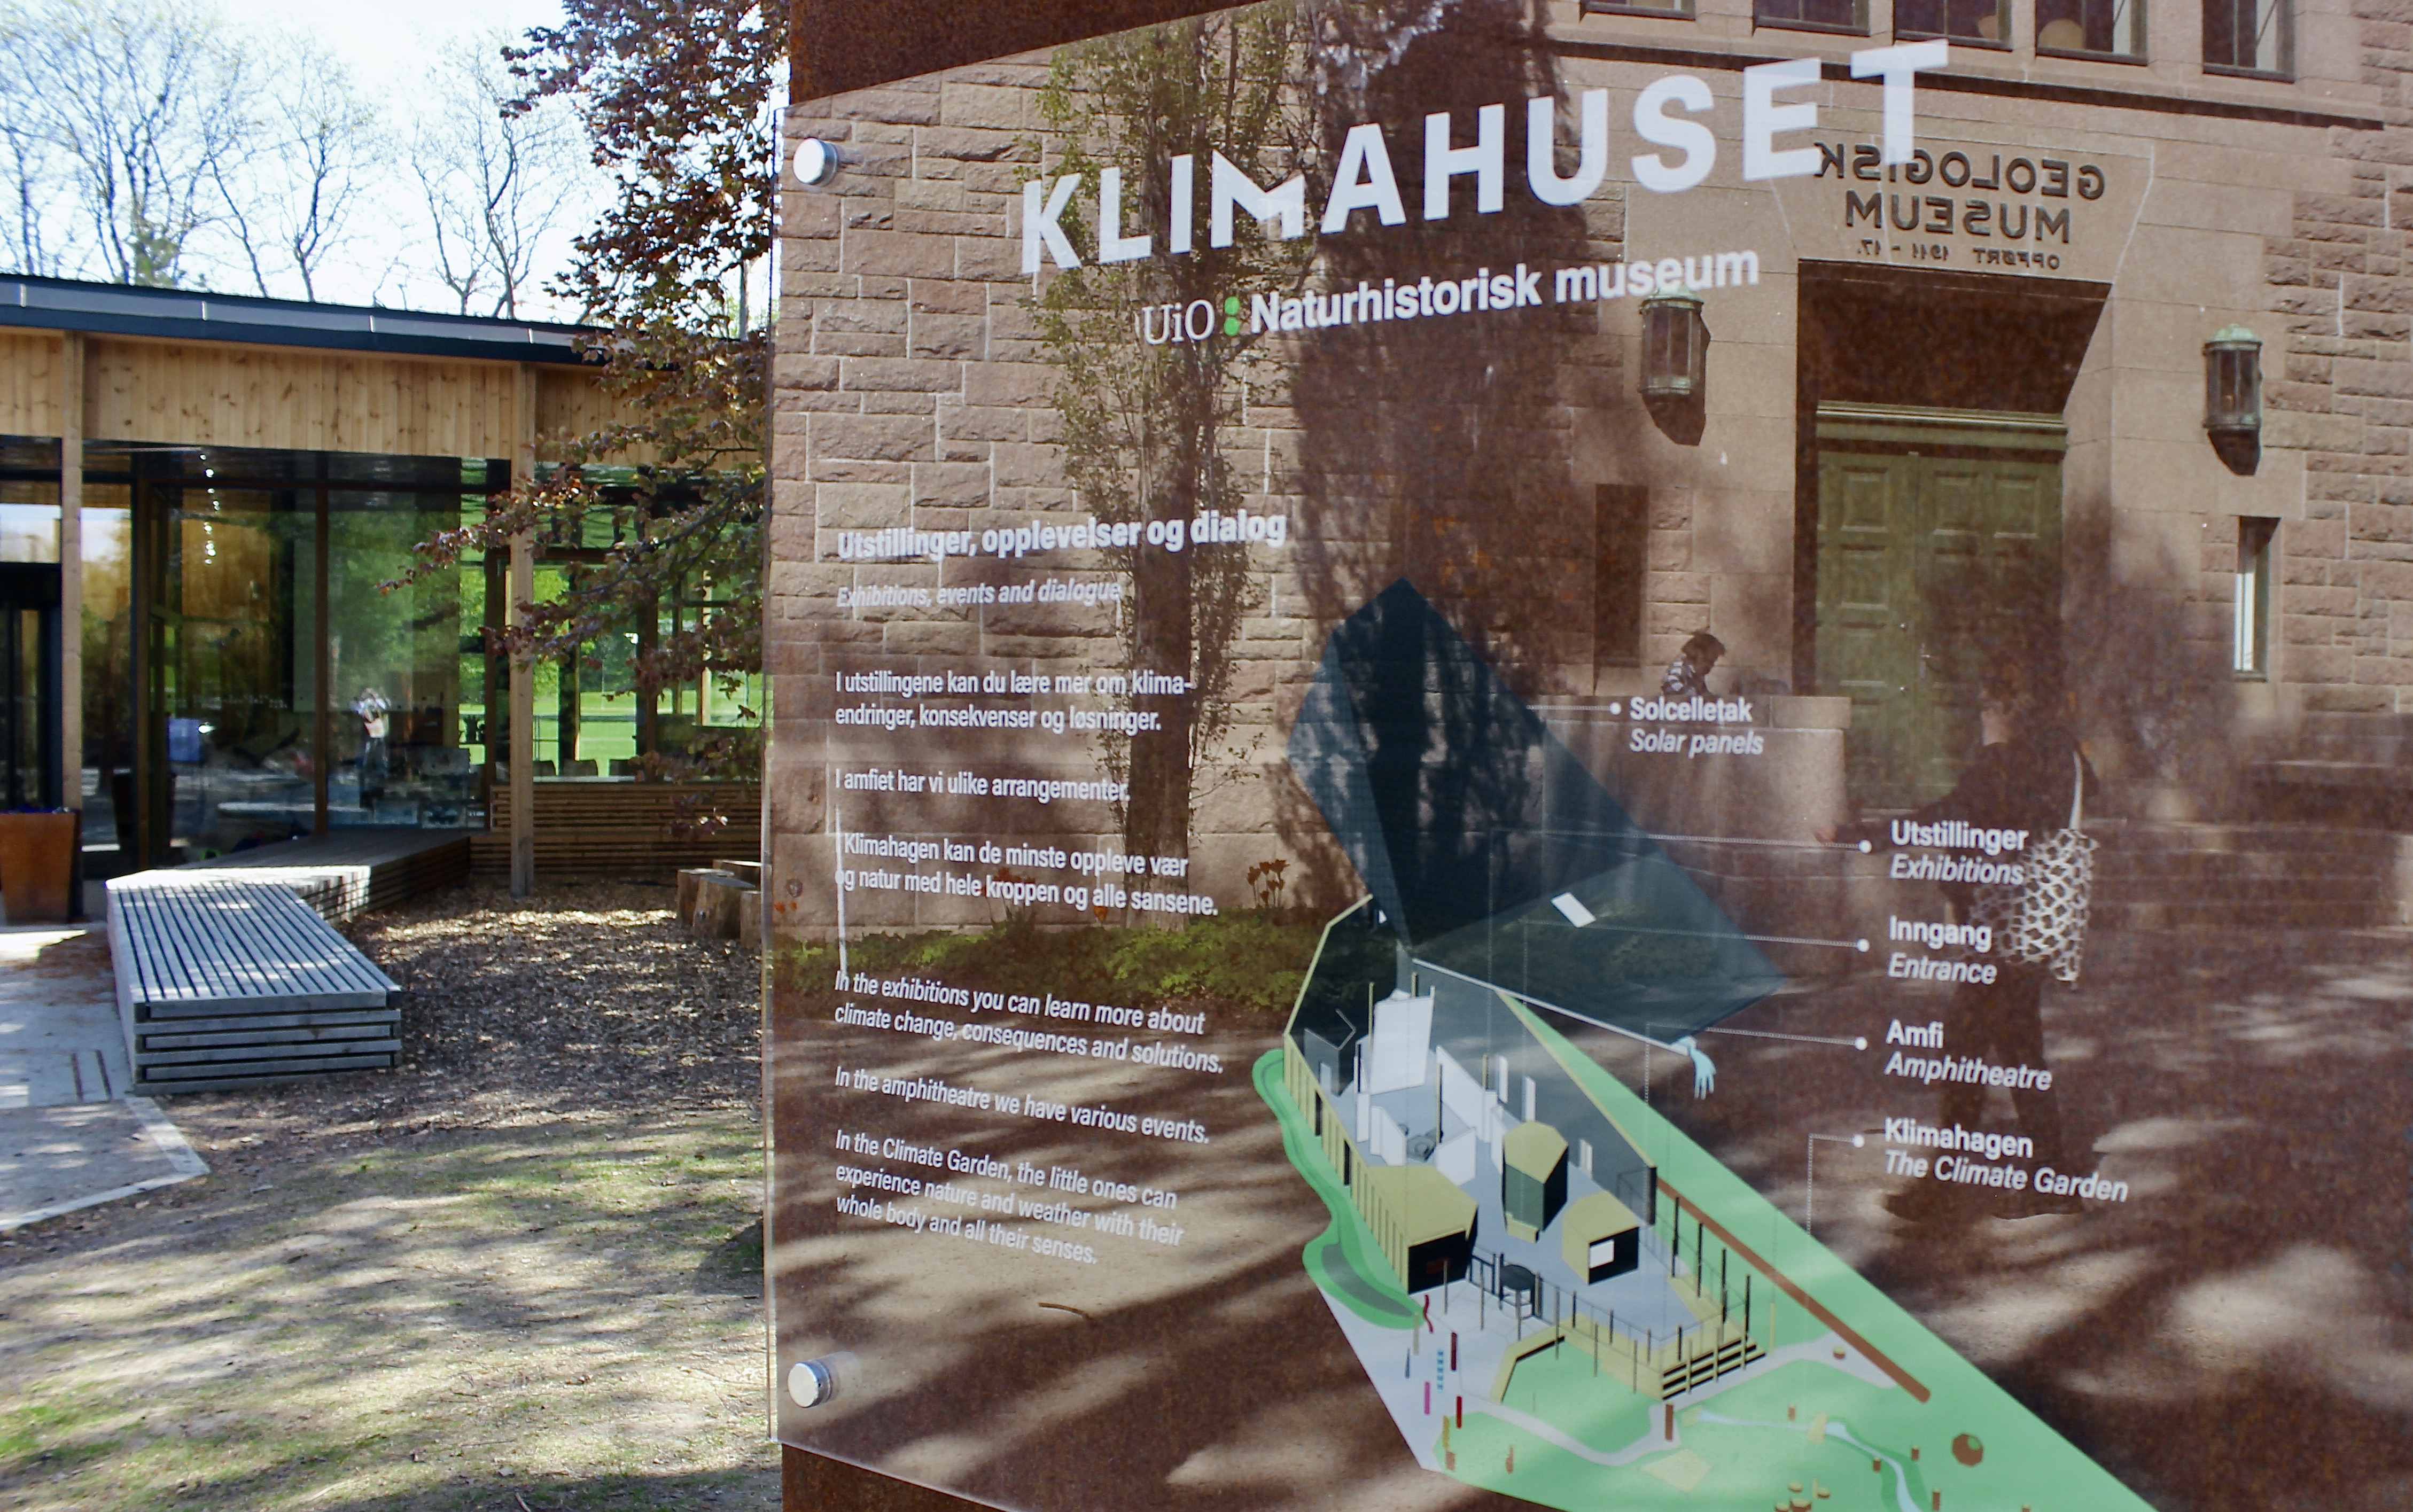
\includegraphics[width=12cm]{pictures/klimahuset/klimahuset_info.JPG}
\caption{Klimahuset entrance area}
\centering 
\end{figure}


\section{Methodology}

My general approach was qualitative in which I conducted (this, this and this). The aim was to generate qualitative data on (this, this and this).

\section{Timeline of events}
In this section I will account for the project timeline, presenting all of the events that make up the project. Me and my research buddies have conducted all of the fieldwork together. Details on each event will be provided in chapter 8: Process diary.

\begin{figure}[H]
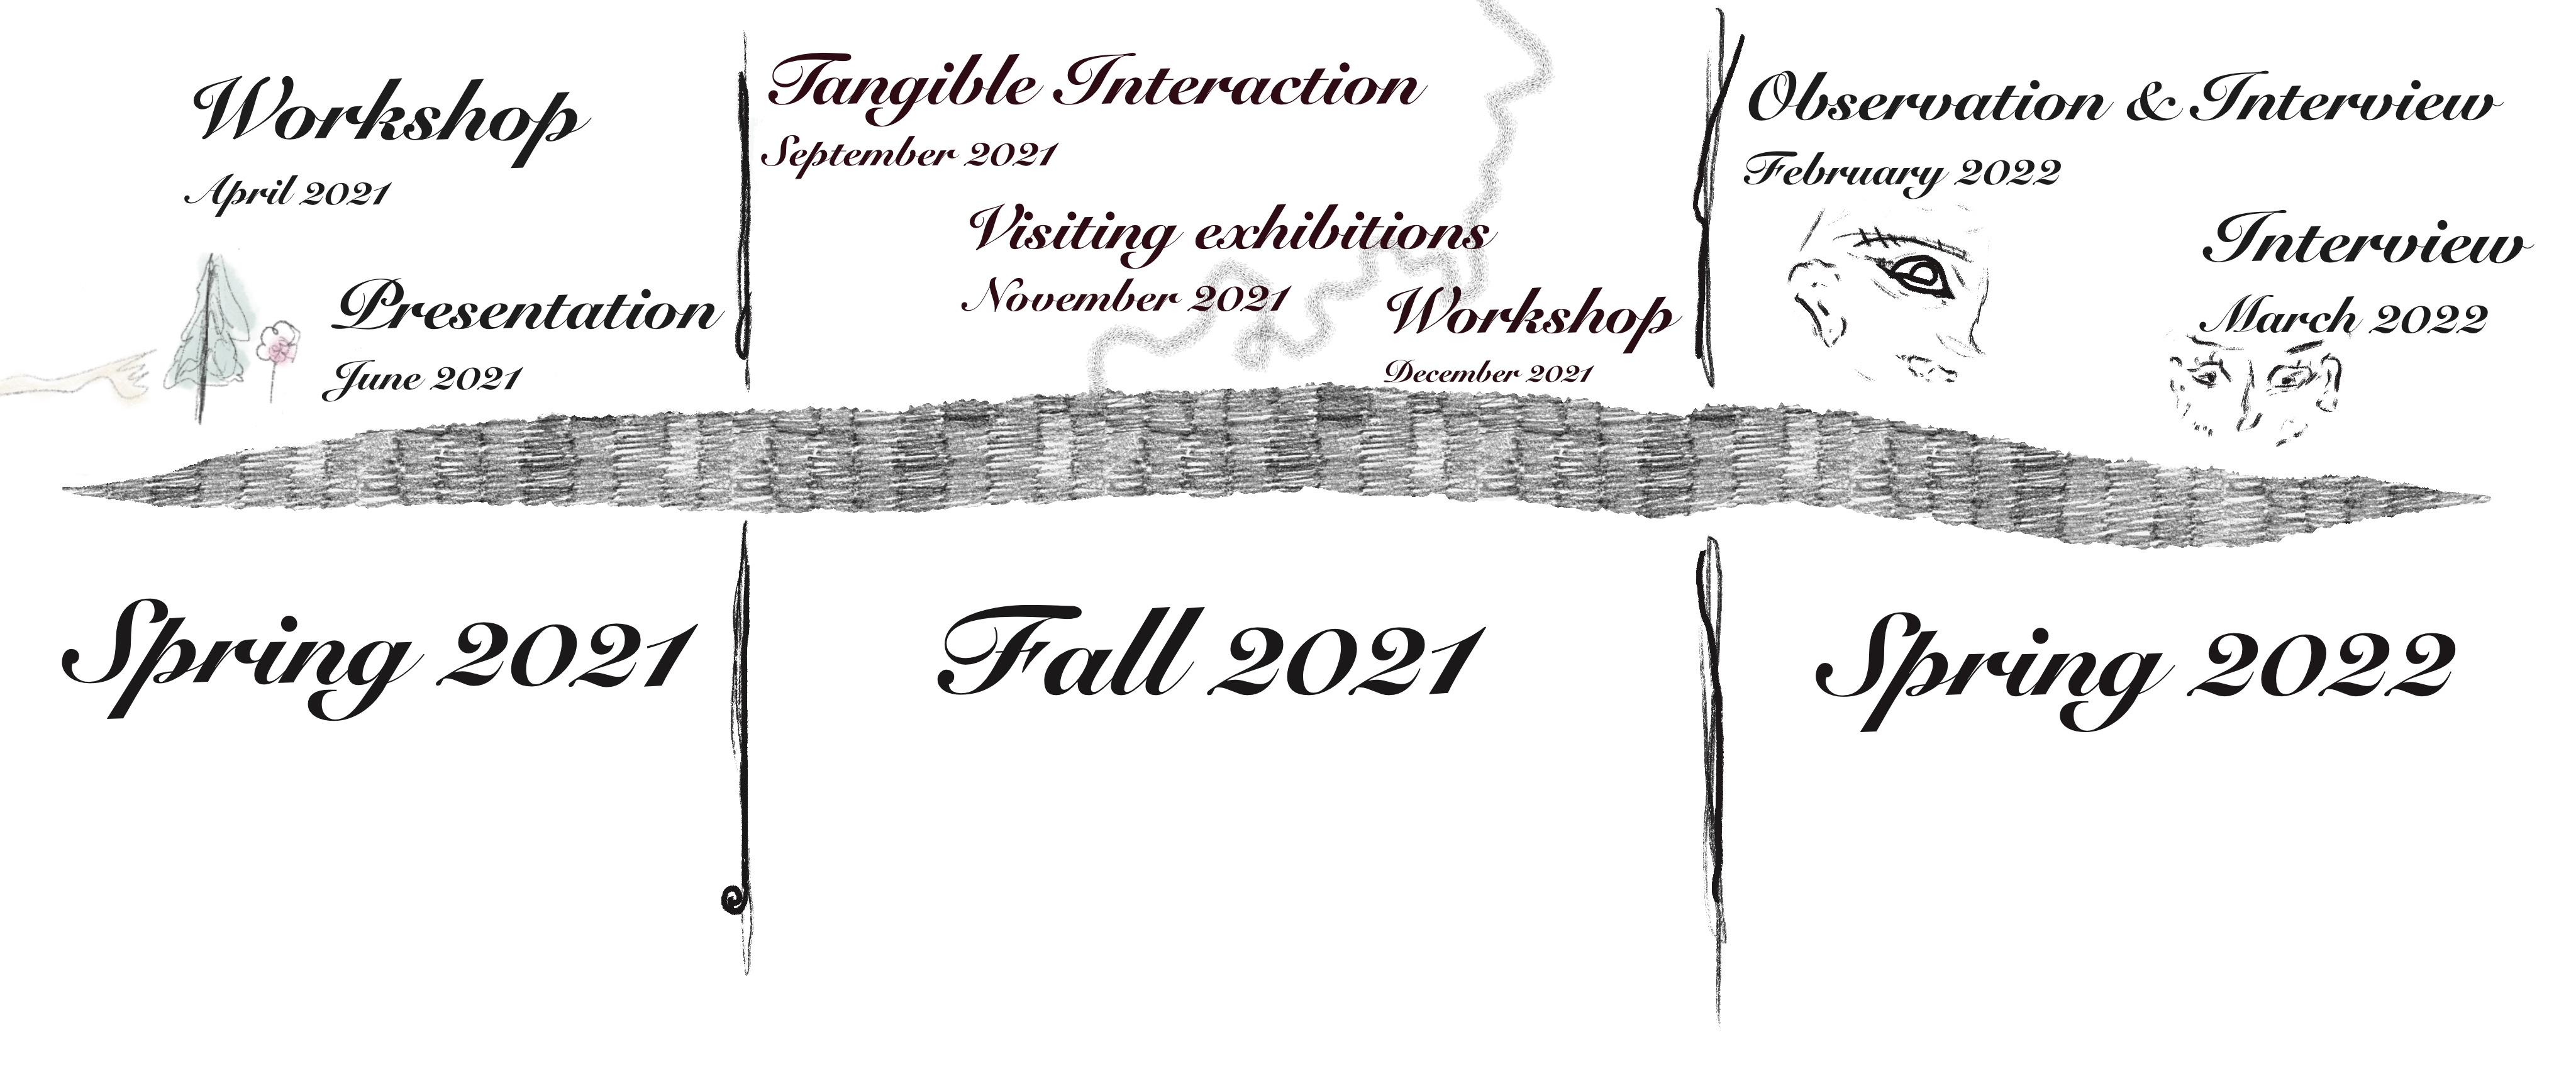
\includegraphics[width=14cm]{pictures/methodology/timeline.jpg}
\caption{Timeline of fieldwork}
\centering 
\end{figure}

The thesis project has been conducted over the course of three semesters. From January- to June spring 2021 I did both theoretical and practical work. In January we met our contact from Klimahuset and had our first viewing and walk-through of the museum's exhibition. Some weeks later we were asked to host a workshop of our choosing that would take place in April. In February I started a literature review focused on getting to know the museum domain, and did so by reading critical literature on exhibition practice \autocite{Thi_book}, on narrative theories and learning in contemporary art museums \autocite{narrative_sitzia}, and on the subject of cultural analysis in museums \autocite{Miekebal_book}, as is evident in chapter 2: The modern museum and Sustainability. To explore the sustainability aspects of the current RQ (\emph{Interactive and visual installations addressing sustainability}), I worked conceptually and explored the topic; a distanced relationship to nature. This later manifested itself in the low-fidelity prototype that was presented at Klimahuset in June 2021. 

All this work contributed to narrow down the research area of interest and in formulating a new research question. 


Next semester, August to December fall 2021, is where most of the practical research efforts were conducted. In September, both me and my research buddies participated in a course about tangible interaction. Through this course we were a part of a team who conceptualised, designed and exhibited an interactive installation during the course duration of one month. Then comes November, where me and my research buddies decided to go to different museums who exhibited interactive installations to experience, observe and collect data on different installations. Late December 2021, my tangible interaction group were requested to exhibit our installation for a group of first-year master students interested in writing about energy-visualisation. And then comes Spring 2022, where the main focus is writing up the thesis. In February we were given the opportunity to observe two school-classes in Klimahsuet, and given a little time to interview with the working Docent's - which we accepted. In March, our supervisor reached out to the Munch museum and giving us the opportunity to interview a concept developer, which we also accepted.

\begin{table}[h]
\centering
\begin{tabular}{l | l}
\textbf{Month} & \textbf{Event}\\
\hline
Jan. 21 & Initial contact and visiting Klimahuset for the first time \\
Feb. 21 & Started literature review on museums \\
Apr. 21 & Hosted a workshop with members of staff from Klimahuset \\
May 21 & Prototyped low-fid installation exploring input through plants \\
Jun. 21 & Held a presentation w/ prototypes at Klimahuset \\
Sep. 21 & Tangible Interaction course: designed an installation \\
Nov. 21 & Visited 5 interactive exhibitions \\
Dec. 21 & Held an energy visualisation workshop with Qi-installation \\
Feb. 22 & Observation of two school children classes in Klimahuset \\
Feb. 22 & Interview with two of Klimahuset's Docents \\
Mar. 22 & Interview w/ concept developer at Munch Museum \\
Apr. 22 & Analysis workshop sessions \\
May 22 & Visited one more interactive exhibition \\
\end{tabular}
\caption{Table of events}
\label{tab:abc}
\end{table}

\section{Research through Design}

When it comes to the structural nature of the coming-together of this thesis, the methodology, I have followed an approach to research practise called Research through Design (RtD).

This research approach was first coined by \autocite{frayling_1994}, in a highly influential paper where he addressed the debate and confusion at the time around what research \emph{is}, what it \emph{involves}, and what it \emph{delivers}. Frayling critiques the stereotypical perceived difference between the Research field and the Art and Design field - whereas 'researching' stereotypically is seen as a cognitive practise, while art and design is seen as an expressive practise \autocite[p. 5]{frayling_1994}. Concluding that since many of the motivations and practises of the two fields are alike, there is a more productive distinction of the relations between research, art and design \autocite[p. 5]{frayling_1994}, namely: research \emph{into} art and design, research \emph{through} art and design, and research \emph{for} art and design. 

According to Frayling, Research \emph{into} art and design is concerned with historical research, aesthetic and perceptual research, and research into theoretical perspectives on art and design \autocite[p. 5]{frayling_1994}. Research \emph{for} art and design on the other hand is research "where the end product is an artefact - where the thinking is, so to speak, \emph{embodied in the artefact}, where the goal is not communicable knowledge in the sense of verbal communication, but in the sense of visual or iconic or imagistic communication"\autocite[p. 5]{frayling_1994}. Lastly, Research \emph{through} art and design is concerned with either/ or materials research, development work (i.e. customising a piece of technology to do something no-one had considered before, and communicate the results), as well as action research (i.e. where a research diary tells, in a step-by-step way, of the experiment and result), underlining how "both the diary and the report are there to \emph{communicate the results}, which is what separates \emph{research} from the gathering of reference materials" \autocite[p. 5]{frayling_1994}.
\par
\textbf{The thing is, during this thesis project I have only done one 'designing' activity (ref. section 8.3: Exploring input through plants), that would suggest a fit into Frayling's description of research through design, as a type of development work. As I hope will become clear, the main reason for this thesis to be placed into the RtD approach by Frayling, is because the process diary and thesis report as a whole documents the subjective, but theoretically grounded progression I (as a researcher) have gone through in terms of gaining knowledge and understanding as to how one can design meaningful interactive experiences in a museum space that addresses sustainability.
}

In the next section I will go through and describe the "steps" (or "moving") I have taken during the thesis project, and how theoretical practise is weighted against (actual) experiences and critical analysis of a set of interactive exhibitions and installations.


\section{How the thesis have developed over time}

I this section I want to give reason as to why and how the thesis research question have changed 




To begin with, the

\section{Model of interaction design research}
Throughout this thesis project, there has been a major directional shift that has affected the research outcome - something which happened right about in the middle of things. I started this thesis project with a pretty clear goal to prototype and design an installation, but have ended up with a critical study of a number of interactive exhibitions and installations that I analyse to identify meaningful relationships or qualities in a museum space. To better show and talk-through this shift, I will use Fallman's model of interaction design research, which I often refer to as 'the design triangle', to better describe how my researching lens have shifted throughout and during the thesis project. It is also a means to explain as to why and how this thesis is fitted and give back to the interaction design research field.

As a design discipline, interaction design’s core can be found in an orientation towards the shaping of digital artefact, products, services, and spaces - with particular attention paid to the qualities of the user experience \autocite[p. 4]{fallman_triangle_2008}. In Fallman’s use of the model, the most interesting and rewarding results in interaction design research come not from taking a specific position in the model, but rather from moving or drifting in between different positions. Thus, as Fallman describe it, "moving in between different positions in the model is, more than anything else, a change of perspective" \autocite[p. 10]{fallman_triangle_2008}.


\begin{figure}[H]
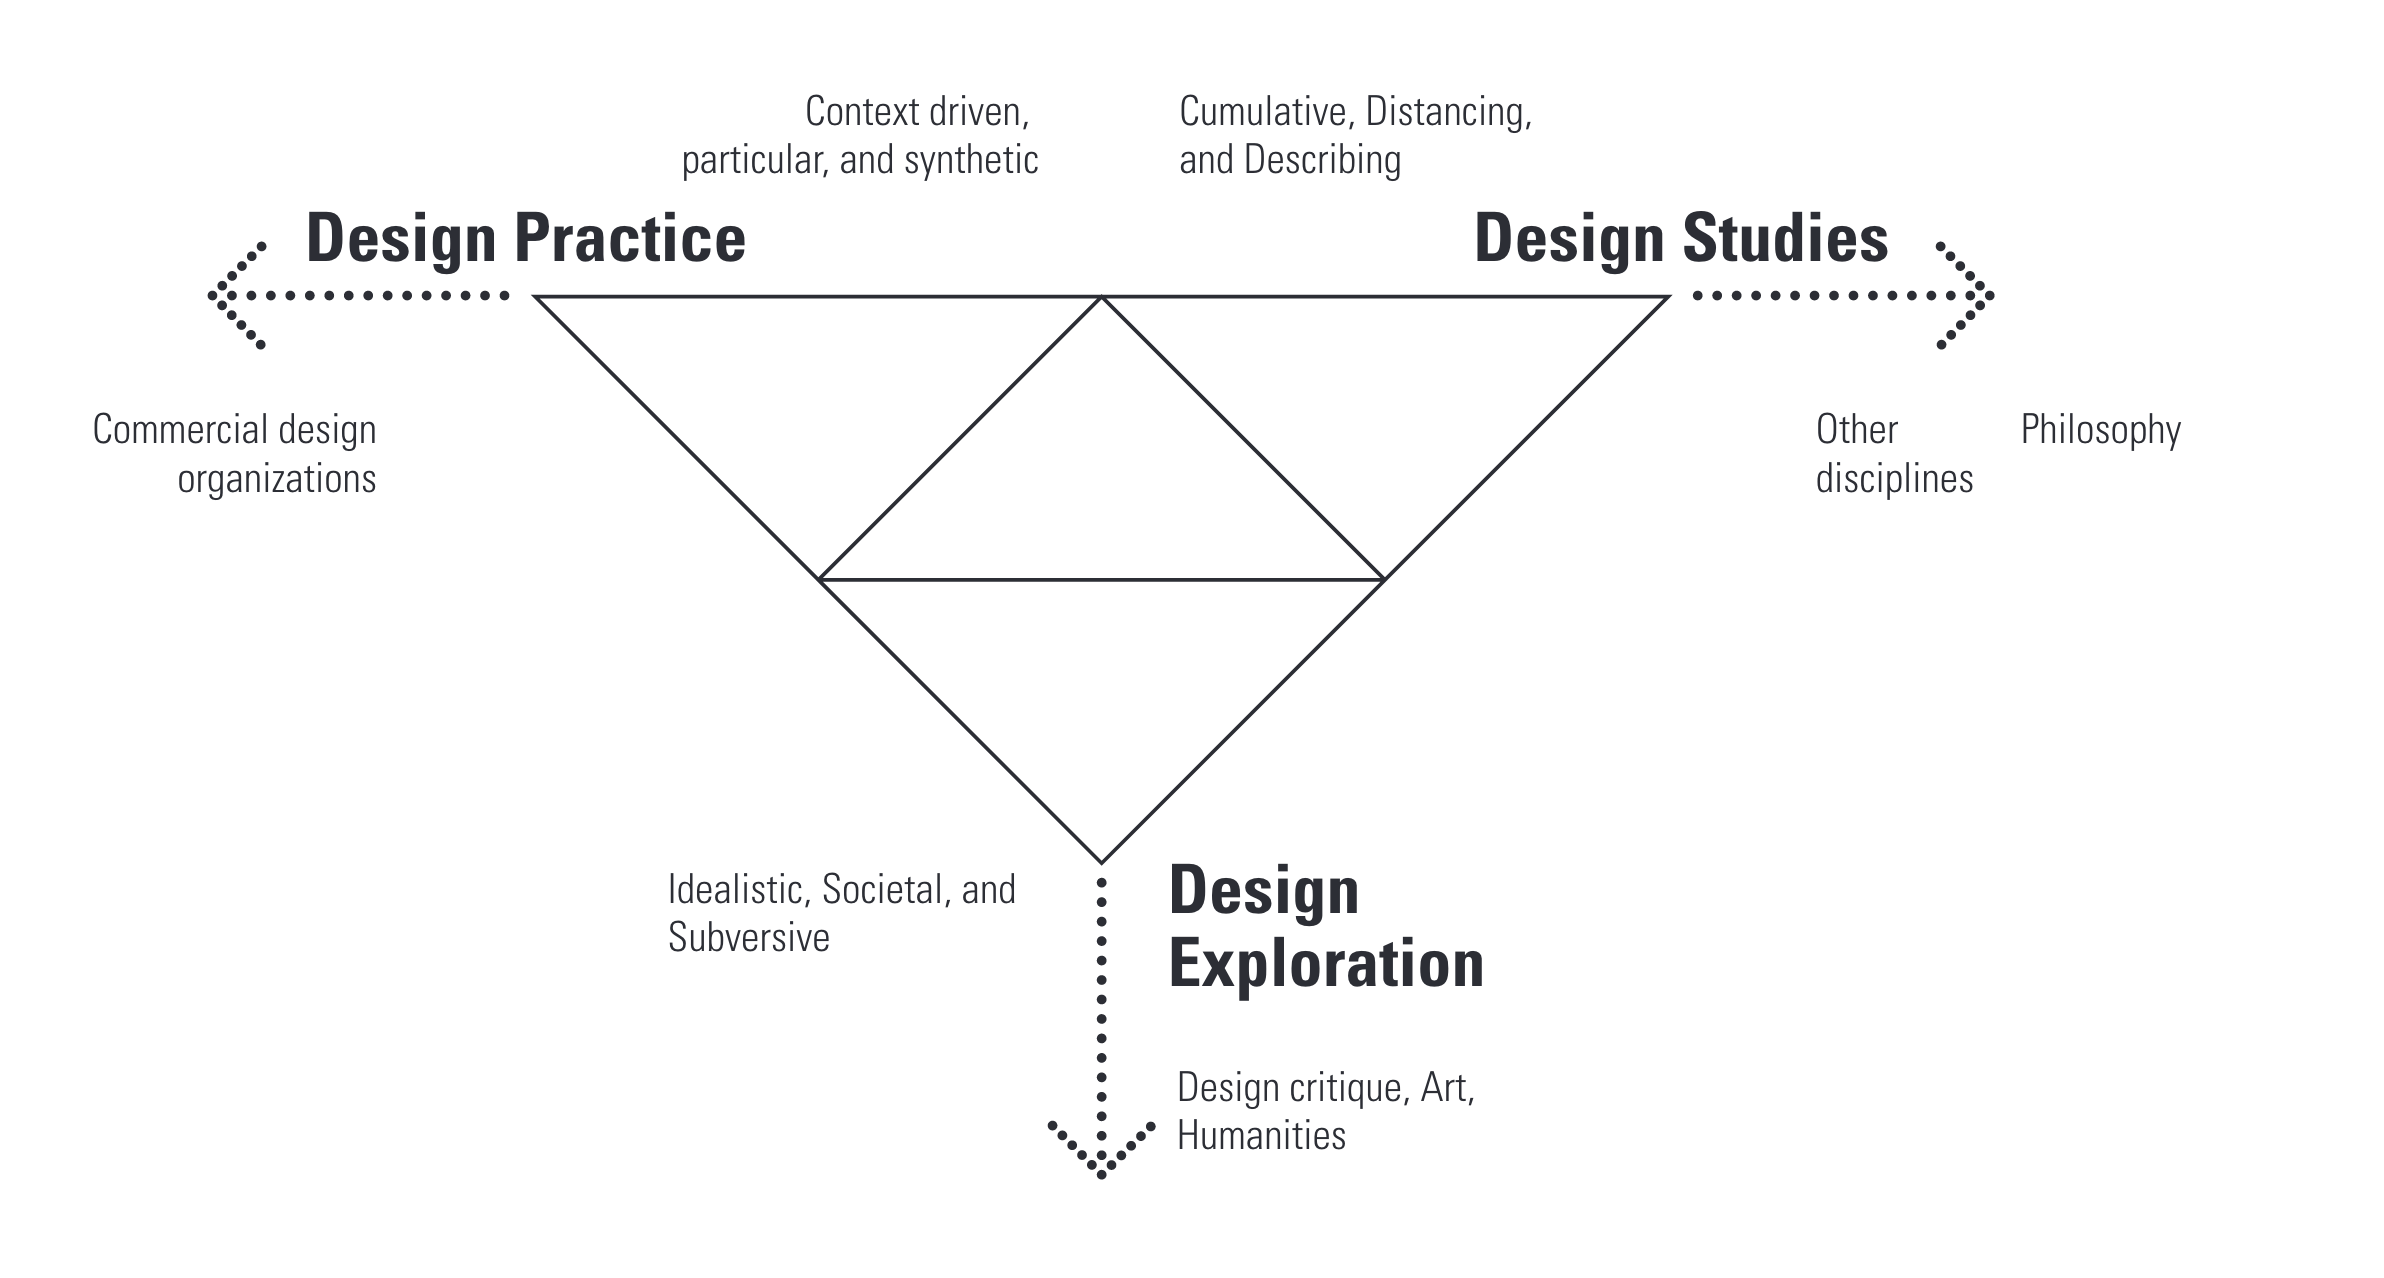
\includegraphics[width=13cm]{pictures/process/triangle.png}
\caption{"The model of interaction design research in its most basic form."}
\autocite[p. 5]{fallman_triangle_2008}
\centering 
\end{figure}

% In terms of doing research through design as a method for interaction design, Zimmerman et. al, explains that what is unique to research though design as an approach, is that it sees the design artefacts as outcomes that can transform the world from its current state to preferred state, which aligns with the domain problems I have accounted for in section 2.0, to address sustainability issues for a more sustainable future. Zimmermann et. al. further explain how the artefacts produced in this type of research become design examples, providing an appropriate channel for research findings to easily transfer to the HCI research and practise communities(Zimmermann et. al, p. 1, 2007).


Design study entails making space for reflections in some kind of structured way on one’s activities: organising reading circles and seminars; and opening up arenas for theoretical, methodological, and philosophical discussions to take place \autocite[p. 18]{fallman_triangle_2008}. The way I have gone forward with this, is to read up on museum practise as evident in chapter 1: Museums, as well as on the topic of sustainability, linking the museum practise up against sustainability. Specifically looking at how sustainability represents a contemporary discourse, and discussing this in relation to how museums want to address and disseminate more contemporary issues to stay relevant. 

+ Design exploration
+ Design Practise


\section{Qualitative research (very unfinished!)}
jeg gjør kritisk forskning: critical design of existing artifacts instead of designing my own. To proper explore Rq I would need t omake a lot of designs, not enough time, better to lean on theory and explore existing installations so that I can actually explore more of them and "talk back to theory". I use theory to analyse installations installations with a design perspective: user experience (meaningful) and dialogical interactive elements/ qualities. 

The paper offers theoretical support for research through design (RtD) by arguing that to legitimise and make use of research through design as \emph{research}, HCI researchers need to explore and clarify how RtD objects contribute to knowledge \autocite[p.2093]{bardzell_immodest_2015}.


Along these lines, Bardzell et.al argue that while the \emph{intentions} of the object's designer are important and annotations are a good mechanism to articulate them, the critical reception of objects can be equally generative of RtD's knowledge impacts \autocite[p. 2093]{bardzell_immodest_2015}.

Bardzell et.al. investigate RtD in its relation to the production of knowledge; specifically, \emph{how design objects are knowledge producers both for those that encounter them and those that design them} \autocite[p. 2093]{bardzell_immodest_2015}. 

To explore how a detailed critique might work when we understand objects as knowledge producers offering to the viewer the possibility to engage in meaning-making practises unfolding a range of complex and multi-faceted views, Bardzell et. al offer a multilevel analysis of a critical design fiction. \autocite[p. 2094]{bardzell_immodest_2015}.

As a field, HCI must answer what sorts of knowledge outcomes can come from objects in (art and) design projects; if we cant, we cannot legitimize RtD as a way of doing HCI research.

My knowledge outcomes from this thesis project:
\begin{itemize}
    \item Proposal of a theoretical lens to read and understand a interactive installations in the museum/ an exhibition. To identify meaningful relations between the dissemination and exhibition practise.
    \item A critical view on the topic of interactivity addressing contemporary topics/issues in a museum space
    \item 
\end{itemize}

This research practise in this thesis is built upon qualitative data through qualitative methods. 

"ethnographic methods" in this thesis: observation, photographic work, interview, conversations, and thinking. 

this thesis has by no means been structured in a read-collect-write linear type of structure.. 

detached researcher? 
What have I been looking for?

Pure subject, what/ who is my subject-object of study?

\section{The role of prototyping in this thesis (unfinished)}

Research through design is a type of research practise where the researcher create artefact- or object prototypes to gain the necessary insight needed to drive and conduct the research project. Prototyping, or the use of prototypes can be used in a variety of ways, and in every stage throughout the project. In the field of human-computer interaction (HCI), software engineering and design, the term prototype is commonly used to signify a specific kind of object used in the design process \autocite[p. 2]{lim_anatomy_2008}. The prototypes are either physical or digital, and function as either a speculative solution, as a manifestation of a design idea, or to explore a design space - all in relation to the research scope and focus. Prototypes are the means by which designers organically and evolutionary learn, discover, generate and refine designs \autocite[p. 2]{lim_anatomy_2008}. They are design-thinking enablers deeply embedded and immersed in design practise, not just as tools for evaluating or proving successes or failures of design outcomes \autocite[p. 2]{lim_anatomy_2008}


In the search for a new way of thinking about prototypes and prototyping, based on the need for exploring and establishing a definition that differs from current approaches in software engineering contexts where engineers use prototypes to identify or satisfy requirements: Lim et. al., conceptualise prototypes as tools for traversing a design space where all possible design alternatives and their rationales can be explored \autocite[p. 2]{lim_anatomy_2008}. In that way, the prototype serves as a communicative manifestation, where the designer is enabled to communicate the rationales of their design decisions through the prototype \autocite[p. 2]{lim_anatomy_2008}. Prototypes stimulate reflections, and designers use them to frame, refine and discover possibilities in a design space \autocite[p. 2]{lim_anatomy_2008}. This new way of thinking about prototypes differs markedly from requirement-oriented approaches like software engineering, recognising design activities as flexible rather than rigid, reflective rather than prescriptive, and problem-setting rather than problem-solving (Schön, 1982). A design idea that satisfies all the identified requirements does not guarantee that it is the best design since a number of ways can meet each requirement \autocite[p. 2]{lim_anatomy_2008}. If the focus of prototyping is framing and exploring a design space, what matters is not identifying or satisfying requirements using prototypes but finding the manifestation that in its simplest form, filters the qualities in which designers are interested, without distorting the understanding of the whole \autocite[p. 2]{lim_anatomy_2008}. In order to support this perspective and to provide a stable foundation for the study of prototypes in HCI, Lim et. al. (2008) proposes a framework for conceptualising prototypes. The framework is an attempt to create an understanding of the nature of prototypes in general and to provide a language for articulating the characteristics of a particular prototype \autocite[p. 3]{lim_anatomy_2008}. Two fundamental aspects of prototyping form the basis of the framework:

1) prototypes are for traversing a design space, leading to the creation of meaningful knowledge about the final design as envisioned in the process of design, and
2) prototypes are purposefully formed manifestations of design ideas.
\autocite[p. 3]{lim_anatomy_2008}

Will answer these:
What values are important in my context?
What is my design outcomes?
What is my design space?
Experience prototyping? Am I going to prototype an experience?
Why and how do I intend a particular prototype to support the design process?



